%
% A simple LaTeX template for Books
%  (c) Aleksander Morgado <aleksander@es.gnu.org>
%  Released into public domain
%

\documentclass{article}
\usepackage[a4paper, top=3cm, bottom=3cm]{geometry}
\usepackage[latin1]{inputenc}
\usepackage{setspace}
\usepackage{fancyhdr}
\usepackage{tocloft}
%
\usepackage{fancyvrb}
\usepackage{graphics} % for pdf, bitmapped graphics files
\usepackage{epsfig} % for postscript graphics files
\usepackage{subfigure,amsmath,array,amsbsy,amsfonts,amssymb}

\newcommand{\inv}{^{-1}}
\newcommand{\tr}{^{\!\top}}
\newcommand{\invtr}{^{-\!\top}}
\newcommand{\diag}{\operatornamewithlimits{diag}}
\newcommand{\argmax}{\operatornamewithlimits{argmax}}
\newcommand{\argmin}{\operatornamewithlimits{argmin}}
\def\R{{\rm I\mkern-3mu R}}




\begin{document}
\pagestyle{empty}
%\pagenumbering{}
% Set book title
\title{\textbf{MATLAB TOOLBOX FOR SMOOTHING AND MAPPING}}
% Include Author name and Copyright holder name
\author{Viorela Ila}



% 1st page for the Title
%-------------------------------------------------------------------------------
\maketitle
% General definitions for all Chapters
%-------------------------------------------------------------------------------

% Define Page style for all chapters
\pagestyle{fancy}
% Delete the current section for header and footer
\fancyhf{}
% Set custom header
\lhead[]{\thepage}
\rhead[\thepage]{}
% Set arabic (1,2,3...) page numbering
\pagenumbering{arabic}
% Set double spacing for the text
\doublespacing



% Not enumerated chapter
%-------------------------------------------------------------------------------
\section{Introduction}
This toolbox implements deferent optimization strategies to solve the simultaneous localization and mapping (SLAM) problem. This is needed to enable autonomous robots to localize, map and navigate previously unknown environments. This work considers smoothing rather than filtering. The advantage is that the estimation errors are reduced by using 
better linearization points. Both, \emph{pose SLAM} (smoothing the robot's trajectory only) and \emph{full SLAM} (estimating the trajectory together with landmarks in the environment) are considered. The user can also chose between \emph{batch} and \emph{incremental} optimization. 
\\
The purpose of the toolbox is to test the mathematics behind the smoothing and mapping algorithms. It is not optimized for speed but still timing of the algorithms is available so that the user can compare different solvers and/or state representations.
\\
The toolbox is available here\\ {\small {\url{https://wiki.laas.fr/robots/ViorelaIla?action=AttachFile&do=view&target=SAMToolbox.tar.gz}}\\ \normalsize It includes three implementations for incremental online smoothing and mapping; a new method of incremental Cholesky updates (called \emph{ L-SLAM}) together with QR factorization of the matrix $A$ (which in the SLAM literature is known as SAM, smoothing and mapping \cite{Dellaert06ijrr}) and the Cholesky decomposition of the matrix $\Lambda$ (based on incremental updates of $\Lambda$ from \cite{Ila10tro}).


% If the chapter ends in an odd page, you may want to skip having the page
%  number in the empty page
\newpage
\thispagestyle{empty}

% First enumerated chapter
%-------------------------------------------------------------------------------
\section{Mathematical background}
%
The SLAM problem estimates the robot trajectory ${\bf x} =\left\{ x_{i}|i\in0..n\right\} $ and the position of landmarks in the environment ${\bf l} =\left\{ l_{j}|j\in1..nl\right\} $  given a set of observations ${\bf z} =\left\{ z_{k}|k\in1..m\right\}$ and control inputs ${\bf u} =\left\{ u_{i}|i\in1..n\right\}$  . Figure~\ref{fig:BN-FG} a) shows the graphical model representation of such a distribution as a Bayes net. In general, for the Bayes net representation we can write the joint density as:
%
\begin{equation}
P({\bf x},{\bf l},{\bf z},{\bf u})\propto P(x_{0})\prod_{j}^{nl} P({\bf l}_{j})\prod_{i}^{n} P(x_{i+1}\mid x_{i},u_{i})\prod_{k}^{m} P(z_{k}\mid x_{i_k},l_{j_k}) 
\end{equation}
%
where $\prod_{j}^{nl} P({\bf l}_{j})$ can be omitted as it is uninformative and the equation above becomes:
%
\begin{equation}
P({\bf x},{\bf l},{\bf z},{\bf u})\propto P(x_{0})\prod_{i}^{n} P(x_{i+1}\mid x_{i},u_{i})\prod_{k}^{m} P(z_{k}\mid x_{i_k},l_{j_k}) 
\end{equation}
\subsection{Factor graph formulation}
%
When the factorization is made explicit we obtain the equivalent factor graph representation of the problem:
%
\begin{equation}
P({\bf x},{\bf l},{\bf z},{\bf u})=\phi(x_{0})\prod_{i}^{n}\psi(x_{i+1},x_{i})\prod_{k}^{m}\varphi(x_{i_k},l_{j_k})
\label{eq:fg}
\end{equation}
 %
In a typical SLAM application, there are three types of factors: the unary factors $\phi(x_{0})\propto P(x_{0})$, odometric factors $\psi(x_{i+1},x_{i})\propto P(x_{i+1}\mid x_{i},u_{i})$  and measurement factors $ \varphi(x_{i_k},l_{j_k})\propto P(z_{k}\mid x_{i_k},l_{j_k})$  and the corresponding graphical representation is shown in Figure \ref{fig:BN-FG} b).
%
\begin{figure}[t]
\begin{center}
\begin{array}{cc}
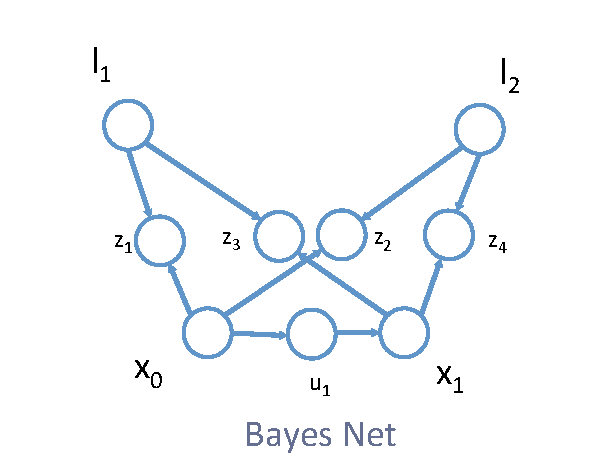
\includegraphics[width=7cm]{figs/BN.pdf} & 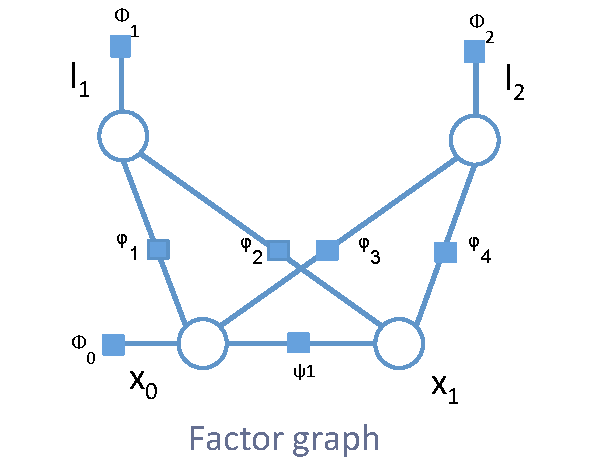
\includegraphics[width=7cm]{figs/FG.pdf}\\
a) & b)
\end{array}
\end{center}
\caption{a) Bayes net representation of SLAM. b) Factor graph representation of SLAM.}
\label{fig:BN-FG}
\end{figure}
%%%%
\subsection{Maximum likelihood estimation}
The optimization problem associated with the full SLAM problem can be concisely stated in terms of a sparse least-squares problem. We want to obtain the maximum likelihood estimate (MLE) for all robot poses ${\bf x}$  and all landmarks ${\bf l}$  collected in vector $\theta=({\bf x},{\bf l})$ :
\begin{equation}
\boldsymbol{\theta}^{*}=\argmax_{\boldsymbol{\theta}}\: P(\boldsymbol{\theta}\mid{\bf z},{\bf u})=\argmin_{\boldsymbol{\theta}}\:\left\{ -\log(P(\theta\mid{\bf z},{\bf u}))\right\} . 
\label{eq:ML}
 \end{equation}
In general, for the SLAM problem, we assume Gaussian distributions and we write:
%
\begin{equation}
\begin{array}{ccc} 
x_i= f_{i}({\bf x}_{i-1},{\bf u}_{i})-{\bf w}_{i} & \Leftrightarrow  & P({\bf x}_{i+1}\mid{\bf x}_{i},{\bf u}_{i})\propto\exp\left(-\frac{1}{2}\parallel f_{i}({\bf x}_{i-1},{\bf u}_{i})-{\bf x}_{i}\parallel_{\Gamma_{i}}^{2}\right)\\
z_k=h_{k}({\bf x}_{i_{k}},{\bf l}_{j_{k}})-{\bf v}_{k}& \Leftrightarrow & P({\bf z}_{k}\mid{\bf x}_{i_{k}},{\bf l}_{j_{k}})\propto\exp\left(-\frac{1}{2}\parallel h_{k}({\bf x}_{i_{k}},{\bf l}_{j_{k}})-{\bf z}_{k}\parallel_{\Sigma_{k}}^{2}\right)
\end{array}
\end{equation} 
%
where $f$  and $h$  are motion and measurement models, $v$ and $w$ are the normally distributed zero-mean motion and measurement noise with covariance matrices $\Gamma_{i}$  and $\Sigma_{k}$, respectively.
%
\subsection{Least-squares problem}\label{subsec:solveSLAM}
Finding the MLE from equation \ref{eq:ML} is done by solving the following non-linear least-squares problem
%
\begin{equation}
\boldsymbol{\theta}^{*}=\argmin \left\{\sum_{i=1}^{n}\parallel f_{i}({\bf x}_{i-1},{\bf u}_{i}) -{\bf x}_{i}\parallel_{\Gamma_{i}}^{2} + \sum_{k=1}^{m}\left\Vert h_{k}({\bf x}_{i_{k}},{\bf l}_{j_{k}})-{\bf z}_{k}\right\Vert _{\Sigma_{k}}^{2} \right \}.
\label{eq:nlls}
\end{equation}
In practice solving this typically nonconvex optimization problem is difficult and prone to local minima. Therefore, non-linear optimization methods such as Gauss-Newton or Levenberg-Marquardt are used to approximate the minimum incrementally, by solving a series of linearized problems. At each iteration, we collect the Jacobian matrices into the matrix $A$ and the current residuals into the right-hand side vector ${\bf b}$ as in \cite{Dellaert06ijrr} ,we obtain the following standard least-squares problem in $\delta$: 
%
\begin{equation}
f(\boldsymbol{\delta})=\frac{1}{2}\left\Vert A\boldsymbol{\delta}-{\bf b}\right\Vert ^{2}
\label{eq:linearEq}
\end{equation}
%
In general, matrix $A$  can be very large, but is quite sparse. In~\cite{Dellaert06ijrr,Kaess08tro} it has been shown that matrix $A$  naturally corresponds to the factor graph representation in equation \ref{eq:fg}. The normalized equation is given by:
%
\begin{equation}
f(\boldsymbol{\delta})=\frac{1}{2}\left\Vert \Lambda\boldsymbol{\delta}-{\boldsymbol \eta}\right\Vert ^{2} 
\label{eq:normalEq}
\end{equation}
%
where $\Lambda=A^{T}A$  is the information matrix and ${\boldsymbol \eta}=A^{T} {\bf b}$  is the information vector. The information matrix $\Lambda$ corresponds to the Markov random field associated with the SLAM problem. We call ``information form'' of the SLAM problem when the state is represented by the information matrix $\Lambda$ and the information vector ${\boldsymbol \eta}$. The information matrix has the advantage of being sparse and remaining of the size of the state $(n+nl)\times (n+nl)$ even if the number of measurements increases.

\subsection{Solving the SLAM problem}\label{subsec:solveSLAM}
To solve the linearized version of equation~\ref{eq:normalEq} we can employ either iterative or direct methods. Each of these families of optimization techniques presents its own advantages and limitations.
%%%%
\subsubsection*{Iterative methods}
Iterative methods, on one hand, only require access to the gradient and have a small memory footprint, but can suffer from poor convergence.
The current state of the art in iterative methods applied to SLAM problem stems from the work
by~\cite{Olson06icra} whose main contribution is a parameterization of the global poses in terms of increments along the trajectory.
Grisetti~\cite{Grisetti07rss,Grisetti10iros} adopted this incremental parameterization as well, but instead defines it on a spanning tree. Both lines of
work use stochastic gradient descent (SGD) to minimize the resulting objective functions in terms of incremental poses.
%%%%
\subsubsection*{Direct methods}
On the other hand, direct methods exhibit quadratic convergence and can be quite efficient for sparse problems like SLAM. 
The linear system can be solved directly either by Cholesky or QR matrix factorizations of the matrix $\Lambda$, respectively
 $A$ and  then performing backsubstitution. 
 \\
\emph{Cholesky factorization} yields $A\tr A =R\tr R$, where $R\tr$ is the Cholesky factor, and a forward and back substitutions on $R\tr {\bf y} = A\tr  {\bf b}$ and
$R\:\theta = {\bf y}$ first recovers ${\bf y}$, then the actual solution, the update $\theta$.
\\
Alternatively we can skip the normal equation in \ref{eq:normalEq} and apply\emph{ QR factorization} directly to the matrix $A$ in \ref{eq:linearEq}, yielding $A = Q\:R$. The solution $\theta$ can be directly obtained by backsubstitution in $R\theta = {\bf d}$ where ${\bf d}=R\invtr\:A\tr\:{\bf b}$. Note that $Q$ is not explicitly formed; instead ${\bf b}$ is modified during factorization to obtain $\bf d$.\\
\\
Recently has been shown in \cite{Konolige10iros} that sparse Cholesky decomposition on $A\tr A$ performs faster than QR decomposition on $A$ . 
%Even if updating $A$ it's more efficient (one block line is added to the matrix every new constraint) than updating $A\tr A$, 
Performing both operations; $A\tr A$ and Cholesky decomposition, on sparse matrices remains more efficient than performing QR decomposition on $A$.
\\
In both strategies, finding the solution involves backsubstitution; if the factor $R$ is sparse, the backsubstitution performs rapidly, but it becomes more inefficient when the fill-in increases. The structure of the factor, in particular the number of non-zero elements in each row and column can be predicted by forming the ``elimination tree''. Forming the elimination tree depends on the chosen elimination ordering. To avoid the fill-in, efficient elimination orderings need to be found. While finding the variable ordering that leads to the minimal fill-in is NP-hard \cite{Arnborg87siam} for general problems, one typically uses heuristics such as the column approximate minimum degree (COLAMD) algorithm by~\cite{Davis04acm}, which provide close to optimal orderings for many problems.

%%%%
\subsection{New method to incrementally update the Cholesky factor}\label{subsec:LSLAM}
The insights gained from the Bayes tree data structure allowed us to develop new simplified incremental algorithms, more suitable to very large scale applications such those in the project ROSACE.
For that we investigated how to incrementally update directly the Cholesky factor $L=R\tr$ in order to combine the advantages of incremental updates and  sparse Cholesky decomposition. 
\\
Integrating a new measurement to the information form is additive. Updating $\Lambda$ and $ {\boldsymbol \eta}$ we obtain:
\begin{eqnarray}
\begin{array}{cc} 
\tilde \Lambda= \left (\begin{array}{cc} 
 \Lambda_{11} & \Lambda_{21}\tr \\
 \Lambda_{21} &  \Lambda_{22}+\Omega
\end{array} \right )\:; & \tilde {\boldsymbol \eta}=\left[\begin{array}{c} {\boldsymbol \eta}_{1}\\ {\boldsymbol \eta}_{2}+{\boldsymbol \omega}\end{array}\right]
\end{array}
\label{eq:updateLambda}
\end{eqnarray}
where $\Omega$ is the increment in information given by $H\tr\:\Sigma_{z_k}\:H$ and ${\boldsymbol \omega}= H\:\Sigma_{z_k}\inv {\bf e_k}$, ${\bf e_k}$ being the prediction-measurement error. Only a part of the information matrix is changed in the update step and the same happens with the lower diagonal factor $L$. The update factor becomes:
\begin{eqnarray}
%
\tilde L= \left (\begin{array}{cc} 
 L_{11} & \\
 L_{21} &  \tilde L_{22}
\end{array} \right )
\label{eq:updateL}
\end{eqnarray}
%
From $\tilde \Lambda = \tilde L\:\tilde L\tr$ and equations \ref{eq:updateLambda} and \ref{eq:updateL} we can write: 
%
\begin{eqnarray}
 \Lambda_{22}+\Omega= L_{21}\: L_{21}\tr  +  \tilde L_{22}\: \tilde L_{22}\tr
\label{eq:L22a}
\end{eqnarray}
%
and the changed part of the $\tilde L$ factor can be computed by applying Cholesky decomposition only to the reduced size matrix:
%
\begin{eqnarray}
 \tilde L_{22}= chol(\Lambda_{22}+\Omega-L_{21}\: L_{21}\tr)
\label{eq:L22b}
\end{eqnarray}
%
%L22_new\(L22*d2+H'*dz);
The part of the RHS: $\tilde {\bf d}=\left[\begin{array}{c} {\bf d_1}\\ \tilde{\bf d_2}\end{array}\right]$ affected by the new measurement can also be easily updated
\begin{eqnarray}
 \tilde {\bf d_2}= \tilde L_{22}\backslash ({\boldsymbol \eta}_{2}+{\boldsymbol \omega} -L_{21}\: {\bf d_1})
\label{eq:L22b}
\end{eqnarray}
%
In an online applications, where the robots are mostly performing exploration task either to map the environment or to navigate towards a specific goal, the new measurements affect variables that are close in the state representation, resulting in small sizes on the information increments $\Omega$  and ${\boldsymbol \omega}$ which translates in efficiency of the update step. Furthermore, in the case of ground robots odometric measurements have higher rate but they only link consecutive robot poses. Therefore adding an odometric measurement can be considered constant time. The constant is $1$ for the particular case of Pose SLAM and $k$ for the case of landmark SLAM, where $k$ is the number of landmarks visible at a time instant.
\\
After updating $\tilda L$ and $\tilda {\bf d}$ backsubstitution is performed to find the solution. 
%By representing the SLAM problem using Bayes trees we learned that during the update process not all the variable are affected and that recovering a nearly exact solution in every step does not require solving for all variables~\cite{Kaess10wafr}. Computational cost can be reduced significantly in this way.
% Translating this to our new method it results in performing the backsubstitution partially. Full backsubstitution starts with the last line of the factor $L$ and goes up to the top, obtaining  the $\boldsymbol \delta$. A partial solving starts from the last variable and continue processing until the change of the variable is lower than a threshold $\alfa$.
\\
%%%%%%%%%%%%
%%%%
\subsection{Optimization on Manifold}\label{subsec:manifold}
The toolbox supports 2D and 3D SLAM. For the 2D the state is represented using $(x,y,\theta)$ and for the 3D the state is representing using $(x,y,z,\phi,\theta,\psi)$. Those are parameterizations of rotation-translation transformation between robot poses in the case of pose SLAM and/or robot position and landmarks in the case of landmark SLAM. Unfortunately those are global parameterizations  which exhibits singularities or other anomalies at various points in the parameter
space. These anomalies can cause serious problems for gradient based minimization procedures, like Gauss-Newton or Levenberg-Marquard.

Optimization problems on a manifold such as SO(3) involves calculating incremental steps in the tangent space to the manifold.

%%%%%%%%%%%%%%%%%%%%%%%%%%
\section{Implementation Details}\label{subsec:Impl}
The toolbox implements and test the SLAM nonlinear optimization problem. To test the 
\subsection{Nonlinear optimization}
Gauss-Newon method:
%--------------------------------------------------------------------
\begin{Verbatim}[frame=single]
Algorithm: Gauss-Newton
i=1;
done=(i>=Solver.maxIT);
while ~done
    [dm,time_solve]=solveSystem(System); 
    done=((norm(dm)<Solver.tol)||(i>=Solver.maxIT));
    if ~done     
        Config=newConfig(Config,dm);
        ck=cputime;
        System=linearSystem(Config,Graph,System);
        i=i+1;     
    end
\end{Verbatim}    
%--------------------------------------------------------------------
Levenberg-Marquard method:
%--------------------------------------------------------------------
\begin{Verbatim}[frame=single]
Algorithm: Levenberg-Marquard

factor=10;
lambda=Solver.lambda;
lambda_max=1e7;
System_new=System;

current_error=10000000;

i=0;
done=0;
while ~done
    i=i+1;
    [S,v]=prepareSystem(System_new.A,System_new.b,lambda);
    %dm=spqr_solve(S,v);
    dm=S\v;
    if ((norm(dm)<Solver.tol)||(i>=Solver.maxIT))
        done=1;
    else
        Config_new=newConfig2D(Config,dm);
        System_new=linearSystem(Config_new,Graph,System_new);
        next_error=norm(System_new.b);  %norm(System_new.A*dm-System_new.b); 
        if(next_error<=current_error)&& (lambda <= lambda_max)
            done =((current_error-next_error)<.005);
            fprintf('.');
            if mod(i,50)==0
                fprintf('\n');
            end
            Config=Config_new;
            current_error=next_error;
            System=System_new;
            lambda=lambda/factor;
        else
            lambda=lambda*factor;
        end
    end
    
end
\end{Verbatim}   
\begin{Verbatim}[frame=single]
function [S,v]=prepareSystem(A,b,lambda)
Atr=A';
H = Atr*A;
v = Atr*b;
D = diag(diag(H));
S =(H+lambda*D);
end
\end{Verbatim}    
%--------------------------------------------------------------------




% Last pages for ToC
%-------------------------------------------------------------------------------
\newpage
% Include dots between chapter name and page number
\renewcommand{\cftchapdotsep}{\cftdotsep}
%Finally, include the ToC
\tableofcontents




\end{document}

